\documentclass[11pt,letter,oneside]{article}
\usepackage{sectsty,setspace} 
\usepackage[top=1.00in, bottom=1.0in, left=1in, right=1in]{geometry} 
\usepackage{graphicx}
\usepackage{epstopdf}
\usepackage{amsmath,latexsym,amssymb,wasysym}
\usepackage[english]{babel}
\usepackage{cite}
\usepackage{citesupernumber}
\usepackage{citecollapse}
\usepackage{wrapfig}
\usepackage{hyperref}
\usepackage{float}
\restylefloat{table}
\usepackage[table]{xcolor} % http://ctan.org/pkg/xcolor
\usepackage{gensymb} % You have to have this to use \degree

\setlength\parindent{0pt} % no indents throughout

\setlength{\abovecaptionskip}{1pt}
\setlength{\belowcaptionskip}{-10pt}
\usepackage[font={small}]{caption}

\parskip=6pt
\pagenumbering{arabic}
\pagestyle{plain}
% squeeze spacey
\linespread{0.99}
\addtolength{\itemsep}{-0.05in}
\usepackage{multicol}
 
\newenvironment{smitemize}{
\begin{itemize}
  \setlength{\itemsep}{1pt}
  \setlength{\parskip}{0pt}
  \setlength{\parsep}{0pt}}
{\end{itemize}
}

\usepackage{fancyhdr}
\pagestyle{fancy}
\fancyhead[LO]{Statement of plans}
\fancyhead[RO]{E. M. Wolkovich}

\newcommand{\Section}[1]{\vspace{-8pt}\section{\hskip -1em.~~#1}\vspace{-3pt}} 


\begin{document}
\bibliographystyle{/Users/Lizzie/Documents/EndnoteRelated/Bibtex/styles/ajhg}
\renewcommand{\refname}{\CHead{}}
\begin{centering}
{\bf Shifting tree growth in response to shifting seasons}\\
\end{centering}
\vspace{1.5ex}
%
% This version is GREAT, but it is also 1700 words (damnit) 
% 
% {\bf Extended summary --} Northern hemisphere forests are critical for healthy ecosystems, healthy people and drive the economies of many countries. Increasingly they are also valued for offsetting fossil fuel emissions, thus mitigating climate change. Yet their immense value is threatened today by multiple risks, including climate change, pests and fire. While extensive research has worked to map and model these threats, the multi-scale and multi-threat nature of forest health has made understanding the major drivers of forest growth and decline difficult. Here, we propose a fellowship to overcome these challenges to produce a continental understanding how, where and why forests are growing or declining. Bridging across disciplines we will develop new models to identify the relative effects of individual-level tree growth processes from stand level properties (e.g. species mixtures) and events (e.g., fire and pest outbreaks), yielding a new understanding of the multiple risks facing forests. Forecasts and visualizations from our work will help guide forest management at the local to federal levels to improve climate resiliency, with global implications for understanding and mitigating climate change itself. 

{\bf Background --} Temperate forests across the globe provide critical resources for people.\cite{oldekop2020forest,costanza2016sustainable} Economically their timber underpins the economies of many states, provinces and countries, with their economic value increasing with climate change through their role in the carbon cycle. Temperate forests currently sequester substantial fossil fuel emissions, offsetting planetary warming and acting as `natural climate solutions'.\cite{pan2011large,griscom2017natural,friedlingstein2022global} The concept of natural climate solutions recognizes the major role that forests play in carbon sequestration and other ecosystem services, including biodiversity maintenance and protection, water quality and stabilizing soils. 

Yet how long forests can continue to offset fossil fuel emissions depends on how they shift their growth in response to the longer, warmer seasons that come with anthropogenic climate change. Fundamentally, longer seasons should allow trees more time to grow and thus increase their growth, an assumption that was previously supported by several studies.\cite{keenan2014net,finzi2020} Recently, however, new work suggests trees do not increase growth with longer seasons,\cite{dow2022}, but why and when this happens is a major open question.\cite{wolkovich2025longer}

{\bf My approach --} My focus on temporal ecology and shifting seasons with climate change (see \emph{Career narrative}) make me well positioned to address this major open question. Further, my current progress on this question, alongside new datasets\cite{zhao2019international,nelson2024x} and advances in modeling approaches,\cite{Carpenter:2017stan,gelman2026bayesian} positions me well to make major progress on it now through a Guggenheim Fellowship. 

\setlength{\intextsep}{6pt} 
\begin{wrapfigure}{r}{0.35\textwidth}
\centering
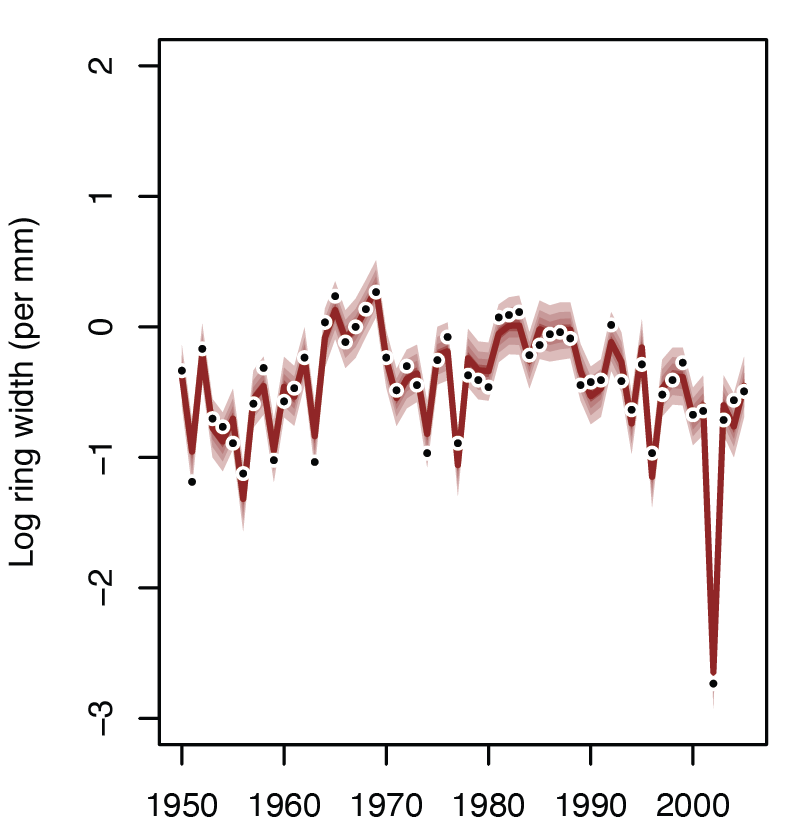
\includegraphics[width=0.33\textwidth]{..//oecd/app2026/figs/ut539_tree22_1panel.png}
\caption{An example of the complexity of tree growth from one \emph{Pinus ponderosa} tree sampled in Utah (USA). Dots show the observed radial growth each year, while the coloring represents estimates from a hierarchical model; shown here is a hierarchical Gaussian process model I may use.\cite{BDA}} 
\label{fig:onetree}
\end{wrapfigure}
Over the past three years I have begun to work in-depth on tree growth, especially through the use of tree rings, which measure radial growth (thicker trunks).  My lab has developed a new image capture machine to rapidly measure tree rings (paper in review by Fong \emph{et al.}), sampled trees across elevation gradients and worked out the major potential reasons we may see variability in tree growth with climate change.\cite{wolkovich2025longer} It seems clear that the likely reasons tree do not grow more with longer seasons are drought stress (not enough water), heat stress (too high temperatures), or species-specific internal constraints (some species are simply conservative in their responses, while others are not). But testing these hypotheses has proved much harder because of the complexity of tree growth. % My lab has developed a new image capture machine to rapidly measure tree rings (paper in review by Fong et al.) and we have worked collaboratively with colleagues at ETH Zurich to sample tree rings across elevational gradients where ...

The forest-level tree growth that drives carbon storage is an emergent property of individual-level tree growth, which is often highly variable and currently difficult to predict (Fig. \ref{fig:onetree}). For these reasons, most work on radial tree growth to date has worked from stand-level averages, after correcting for age-trends (tree-level allometry).\cite{cook1985time,Schofield2016} This approach has been powerful for understanding long-term large-scale patterns of tree growth.\cite{williams2020large} But it has also made it difficult to identify how longer, warmer seasons affect tree growth. Understanding how longer seasons affects tree growth requires modeling drivers of variability in the time-series of individual trees (Fig. \ref{fig:onetree}) and then build up to understand how different species and stands (sites) respond to longer seasons alongside climate. It effectively requires an entirely new approach to modeling tree growth. 

{\bf Methods --} For my Guggenheim fellowship I propose to develop new models of tree growth that can tease apart how longer seasons, alongside shifting climate, have impacted diverse forests across North America. I have already begun preliminary work on these models (Fig. \ref{fig:onetree}) and am well positioned to complete them for trees across North America during my fellowship. 

I propose to work with a leader in hierarchical modeling (Andrew Gelman, Columbia University)\cite{BDA} and an expert in tree growth and drought (Dr. Benjamin Cook, NASA-GISS/Monash University) to understand how tree growth and forests have shifted in recent decades with longer seasons, and project shifts in the future. I will use tree ring data from the International Tree Ring Data Bank \cite{zhao2019international}, and climate data from PRISM and NASA to model tree growth across North America since 1896 (start date of of robust gridded climate data). We will estimate the start and end of the growing season using newly available gridded data.\cite{nelson2024x} For climate, I plan to begin by focusing on summer warmth through growing degree days (GDD), moisture (and thus drought) estimated through precipitation sums and stress effects of both heat and drought possible through high vapor pressure deficit (VPD). Given the different climate drivers in western versus eastern North America, I plan a multi-step approach: I will fit data from western North America first where winter precipitation and VPD often dominate as drivers, then I will fit data from eastern North America where GDD is likely more important. Multiple aspects of my proposed work make it highly feasible, including the scientific backgrounds, interests and skills of myself and proposed collaborators (Gelman and Cook), as well as extensive work to compile data and design a plan that can be rapidly achieved.

{\bf Impact --} My focus on climate will be critical for understanding how longer seasons affect tree growth outside of the shifting climate that drives longer seasons. Further, it will allow me to forecast from my model to predict how forests will respond to continuing anthropogenic climate change. These forecasts will be especially unique in providing guidance on how forest health may shift depending on species and age composition (both of which can be managed through forest policy) and the management of fire and pest outbreaks. My approach will yield a multi-level and multi-risk view, highlighting areas where management and policy could affect outcomes, yielding more resilient forests.
 % In addition to the scientific excellence brought by Gelman, additional collaborators have already pledge support the project with finalizing data (Dr. Cook, mentioned above) and helping with computational and modeling issues (Dr. Bob Carpenter). Further, Columbia University has agreed to provide all necessary support to make sure the project is a success, including office space, compute and additional resources as needed.

This project will shift our fundamental scientific understanding of how trees grow, yielding our best estimates of radial growth responses to climate---and how growth shifts with longer seasons. The work during my fellowship will lead to 1-2 papers in high profile scientific journals (e.g., \emph{Science, Nature}) and likely high media coverage, which I have often received for my work. Beyond, I expect this new outlook on tree growth will lead to new experiments, studies and drive new knowledge. Additionally, multiple aspects of my approach are designed to extend beyond. My multi-scale approach can be extended both outward---to forests in other regions, countries and continents---and temporally downscaled, moving beyond annual resolution to potentially drawing on weekly or daily data (increasingly available through dendrometer networks). Both areas I hope to expand to after my fellowship period. 
\newpage
\pagenumbering{gobble}
{\bf Bibliography}
\begin{footnotesize}
\def\section*#1{}
\bibliography{/Users/Lizzie/Documents/git/bibtex/LizzieMainMinimal}
\end{footnotesize}

% \emph{Rational for host institutions}\\

% (I expect at least one paper in \emph{Nature Climate Change} or similar, one methods and conceptual paper in a high-profile climate change focused journal so that the method can be widely used for other crops and wild species, as well as potentially one paper specific to winegrapes research)


\end{document}



{\bf Timeframe --} % schedule/timeline
The fellowship is proposed for 15 September 2027 to 29 February 2028 (24 weeks) to bring Professor Wolkovich to Columbia University to work with Andrew Gelman and collaborators. If funded, we plan several videoconference meetings to discuss the aims, data and some modeling decisions in advance. Data collection and cleaning will then start before the fellowship to maximize the in-person time. While the project is ambitious, we (Wolkovich and Gelman) have worked together on the proposed design and aims to make sure it is achievable within the 6-month time-frame, and expect to have a report and at least one draft publication ready by the end of the CRP Fellowship. 

{\bf September 2027:} Finalize merging and cleaning tree ring and climate data. Gather mapping layers for forest pest and fire \cite[e.g.,][]{pane2026spatial,williams2025western}. Finalize model approach.\\
{\bf October-November 2027:} Develop models, including code and checking, fit empirical data for North America (likely first to western areas, then extend to east).\\
{\bf December 2027:} Posterior predictive checks \cite{gelman2026bayesian} for North America, and begin to work on visualizations for communication and dissemination.\\
{\bf January-February 2028:} Forecasting from model, including testing and finalizing visualizations for communication to stakeholders. Prepare publication and final report. 


